\documentclass[12pt,a4paper]{article}
\usepackage{algorithm, algpseudocode, amsmath, amssymb, caption, csquotes, empheq, geometry, graphicx, hyperref, listings, multirow, physics, siunitx, subcaption, upgreek}
\usepackage[section]{placeins}

\title{Computational Physics\\Problem Set 2}
\author{Saleh Shamloo Ahmadi\\Student Number: 98100872}
\date{September 27, 2021}

\hypersetup{colorlinks=true}

\newcommand{\juliafigpath}{../fig/julia}
\newcommand{\rbdfigpath}{../fig/random-ballistic-deposition}

\begin{document}
	\maketitle
    \section{Julia Set}
    Informally, The Julia set of a complex mapping function consists of the points in the complex plane that
    do not diverge after repeatedly applying the mapping function to them. That is, if $z_{n + 1} = f(z_n)$ the
    Julia set $J(f)$ consists of the points where the sequence $z_n$ converges if $z_0$ is the point.

    To find $J(f)$, we first find a lower bound for the abolute value of numbers that diverge ($R$)
    (this just has to be \emph{a} lower bound, not \emph{the smallest} lower bound). Then we repeatedly apply
    the mapping $f(z)$ to the points $\abs{z} < R$ and stop when $\abs{z_n} > R$. For better visuallization of
    the function's behavior, we color each point based on the iteration in which the point diverged.
    Algorithm \ref{alg:julia} demonstrates this in practice.

    \begin{algorithm}
        \caption{Fractal Generation by Relative Mapping}
        \label{alg:julia}
        \begin{algorithmic}[1]
            \Function{fractal}{$f, i_{max}, R$}
            \Comment{$f$ is the mapping function and $i_{max}$ is the maximum iteration depth}
                \ForAll{$z$ in the complex plane, with a given resolution}
                    \State $i \gets 0$
                    \While{$i < i_{max}$ \textbf{and} $\abs{z} < R$}
                        \State $z = f(z)$
                        \State $i \gets i + 1$
                    \EndWhile
                    \State $J[z] \gets i$
                    \Comment{$J$ is the array holding the divergence iteration for each point of the complex plane
                    and $J[z]$ is the element corresponding to the complex number $z$}
                \EndFor
                \State \textbf{return} $J$
            \EndFunction
        \end{algorithmic}
    \end{algorithm}
    The quadratic polynomial $f(z) = z^2 + c$ is of particular interest. It is related to the mandelbrout set.
    The polynomials in this report are all generated using this mapping function.
    \begin{figure}
        \centering
        \makebox[\linewidth][c]{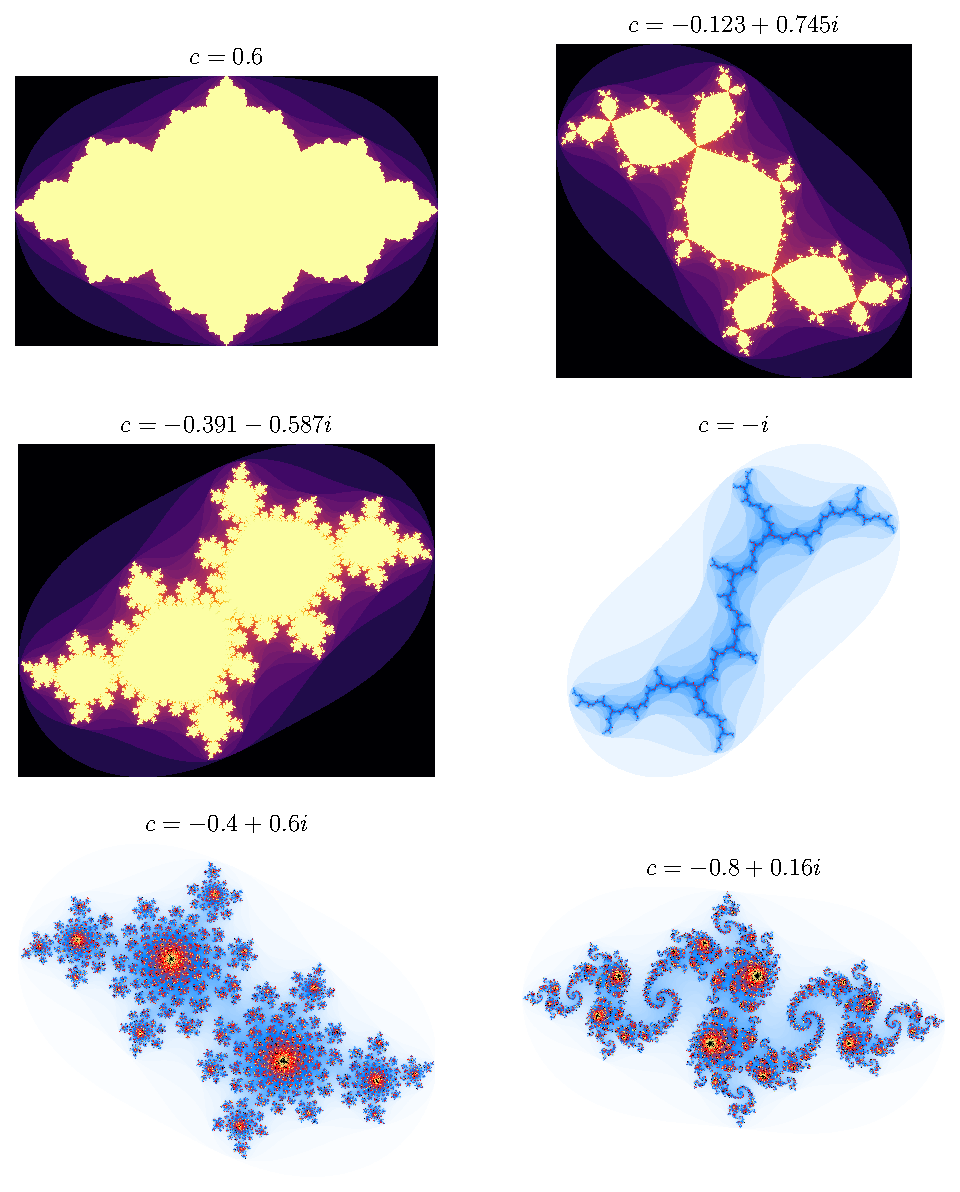
\includegraphics{\juliafigpath/julia-main}}
    \end{figure}
    \begin{figure}
        \centering
        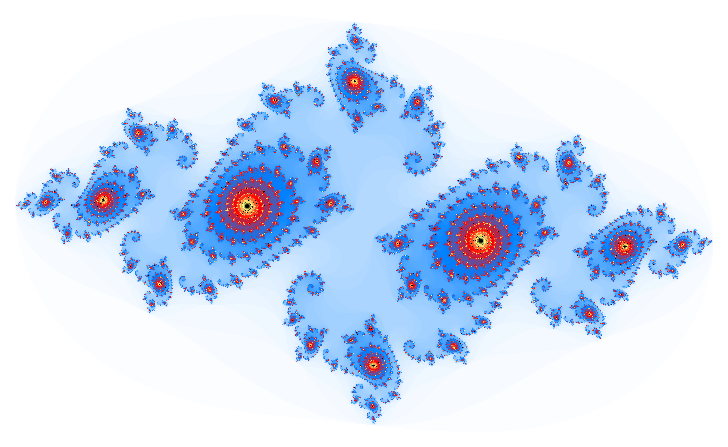
\includegraphics[width=\linewidth]{\juliafigpath/julia-spiral}
    \end{figure}
    \begin{figure}
        \centering
        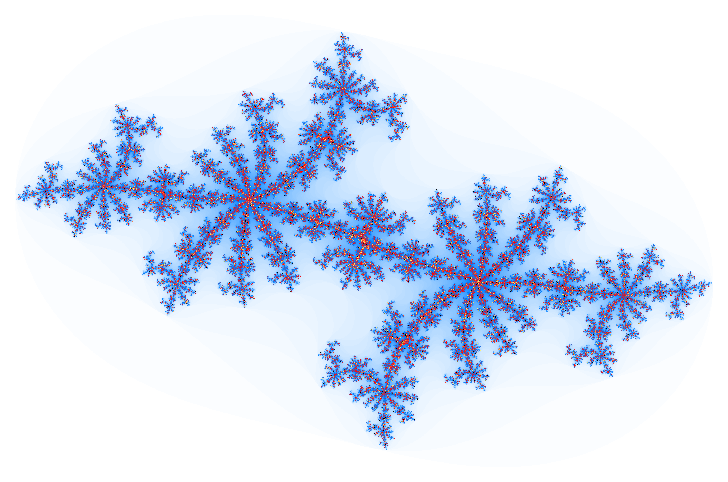
\includegraphics[width=\linewidth]{\juliafigpath/julia-frost}
    \end{figure}
    \begin{figure}
        \centering
        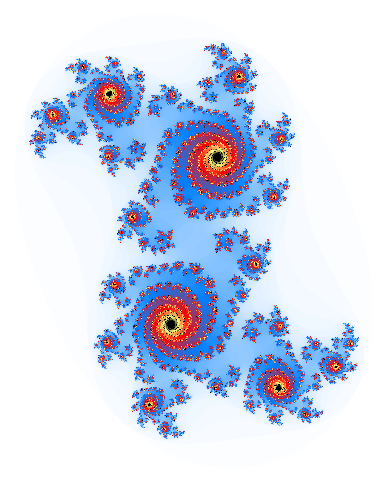
\includegraphics[width=\linewidth]{\juliafigpath/julia-galaxy}
    \end{figure}
    \begin{figure}
        \centering
        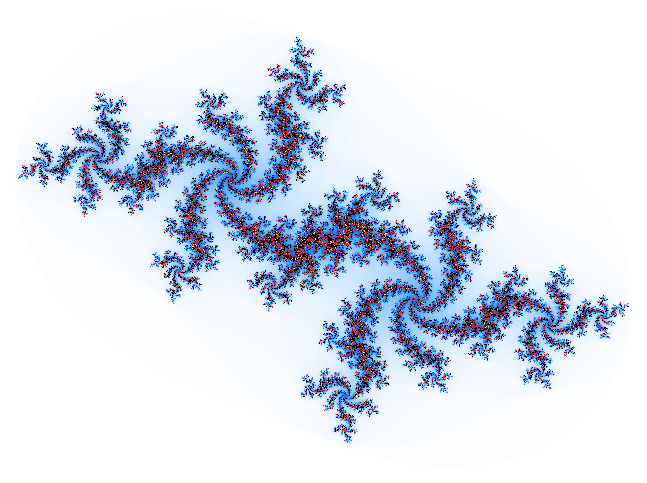
\includegraphics[width=\linewidth]{\juliafigpath/julia-pentapod}
    \end{figure}
    \begin{figure}
        \centering
        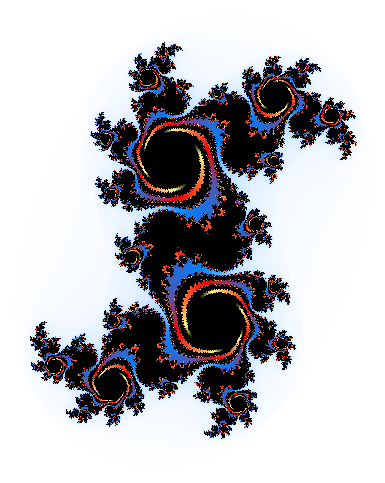
\includegraphics[width=\linewidth]{\juliafigpath/julia-chaotic}
    \end{figure}
    \begin{figure}
        \centering
        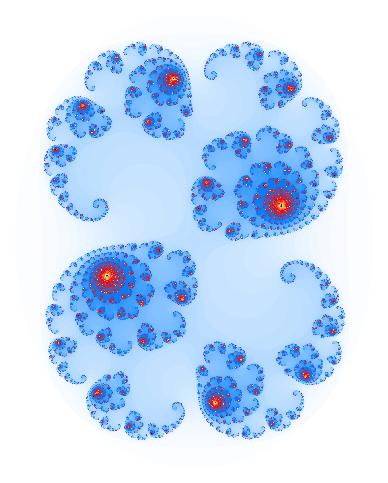
\includegraphics[width=\linewidth]{\juliafigpath/julia-reverse-s}
    \end{figure}
    \section{Random Ballistic Desposition}
    The algorithm for random ballistic desposition is trivial; Just add points particles to different points (buckets)
    randomly and save your data in consistent intervals.
    
    \begin{figure}[htb!]
        \centering
        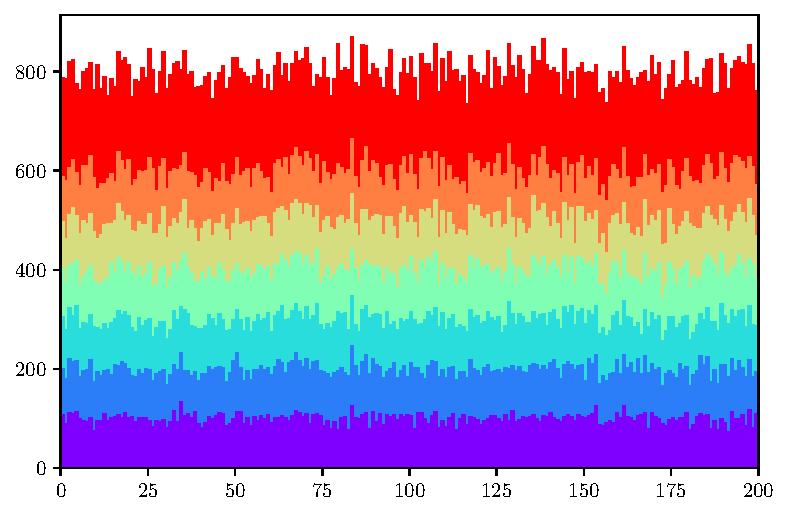
\includegraphics[width=\linewidth]{\rbdfigpath/vis}
    \end{figure}

    To check the validity of our data, we can use simple linear regression. If the particles are randomly deposited,
    their final distribution must be uniform. So
    \begin{equation}
        \bar{h}(t) = \frac{\sum_{i=0}^{L}h_i(t)}{L} = \frac{t}{L},
    \end{equation}
    where $L$ is the length of the 1D surface, $h_i(t)$s are the heights (number of deposited particles) of each point
    at time $t$, and $\bar{h}(t)$ is the average height at time $t$.

    \begin{figure}[htb!]
        \centering
        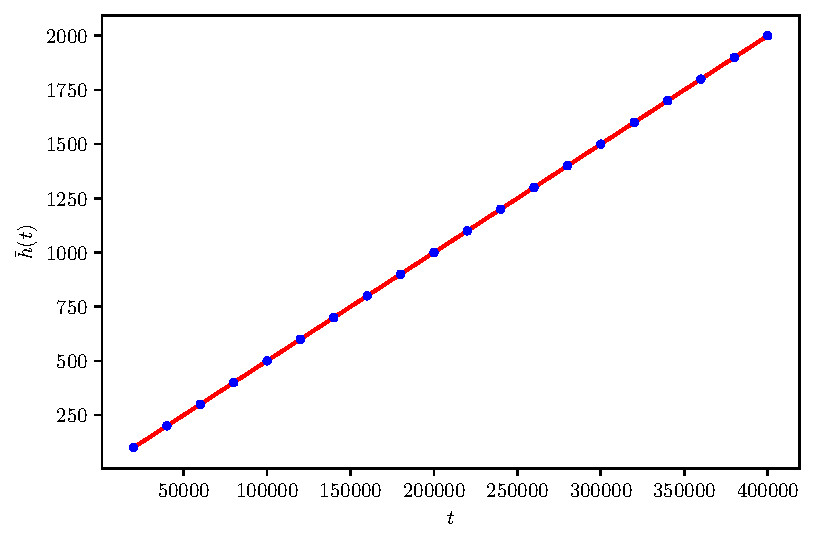
\includegraphics[width=\linewidth]{\rbdfigpath/means}
        \caption{$L = 200$, $\text{slope} = 0.005 \pm \num{5e-19}$}
    \end{figure}

    We can also calculate the \emph{dynamic growth exponent}; In the following equation, $\beta$ is the
    dynamic growth exponent ($\mathrm{SD}$ is the standard deviation):
    \begin{equation}
        \mathrm{SD}_h(t) \sim t^\beta
    \end{equation}
    After running the simulation multiple times and also with larger number of points and larger time,
    it is obvious that $\beta$ oscillates around $0.5$.

    \begin{figure}[htb!]
        \centering
        \begin{subfigure}{\linewidth}
            \centering
            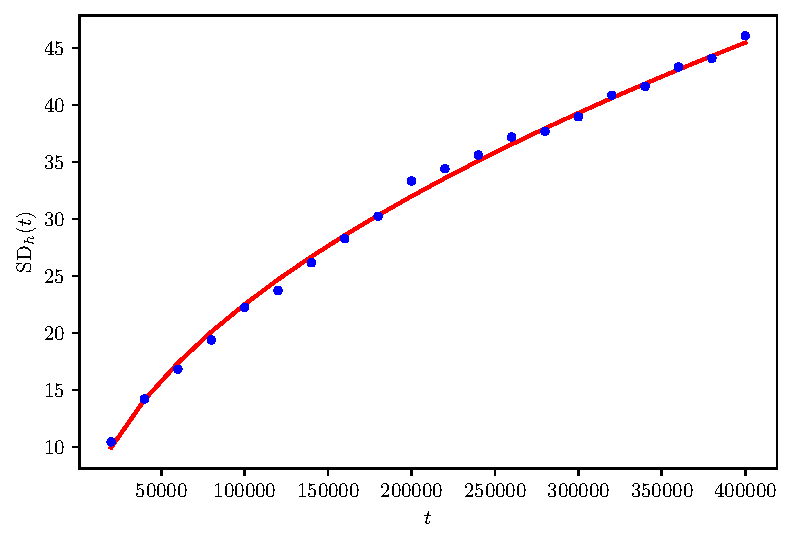
\includegraphics[width=\linewidth]{\rbdfigpath/deviations}
        \end{subfigure}
        \begin{subfigure}{\linewidth}
            \centering
            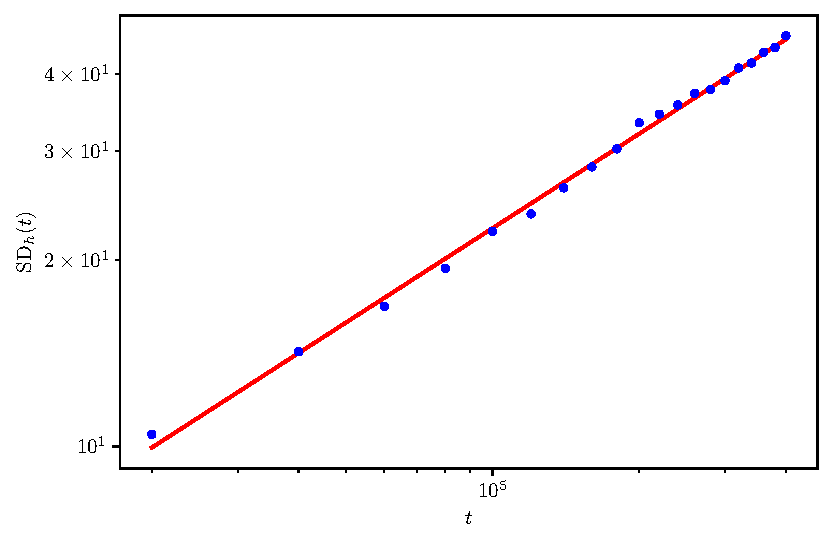
\includegraphics[width=\linewidth]{\rbdfigpath/deviations-loglog}
        \end{subfigure}
        \caption{$\beta=0.507 \pm 0.007$}
    \end{figure}
\end{document}
